% Основные настройки документа
\documentclass[8pt]{beamer} % Тип документа и размер шрифта
\usepackage[english, russian]{babel} % Используемые языки
\usepackage[T1, T2A]{fontenc} % Кодировка кириллицы
\usepackage[utf8]{inputenc} % Кодировка исходного файла
\usepackage{siunitx} % Работа с величинами
\usepackage{tikz} % Построение графиков из .csv-файлов
\usepackage{pgfplots} % Оформление графиков

% Настройки оформления
% Базовые настройки темы презентации
\usetheme{AnnArbor} % Тема компоновки элементов
\usecolortheme{beaver} % Встроенная цветовая тема
\usefonttheme{serif} % Начертание шрифта
\setbeamertemplate{navigation symbols}{} % Отключение элементов навигации
\mode<presentation>

% Индивидуальная цветовая палитра
\definecolor{gold}{rgb}{0.86, 0.635, 0.369} % Золото #DCAD76
\definecolor{blue}{rgb}{0.2, 0.6, 0.6} % Синий #339999
\definecolor{darkblue}{rgb}{0.086, 0.412, 0.478} % Темно-синий #16697A
\definecolor{red}{rgb}{0.756862745098039, 0.070588235294118, 0.117647058823529} % Красный #C1121F
\definecolor{yellow}{rgb}{1, 0.718, 0.012} % Желтый #FFB703
\definecolor{Color6}{rgb}{0.0667, 0.5412, 0.6980} %#118AB2 
\definecolor{Color7}{rgb}{0.1490, 0.2745, 0.3255} %#264653
\definecolor{Color8}{rgb}{0.5529, 0.6000, 0.6824} %#8D99AE
\definecolor{Color9}{rgb}{0.9059, 0.4353, 0.3176} %#E76F51
\definecolor{Color10}{rgb}{1, 0.7059, 0.6353} %#FFB4A2

% Индивидуальные настройки темы
\setbeamercolor{title in head/foot}{fg=gold}

\setbeamercolor{sections/subsections in toc}{bg=gray}
\setbeamercolor{sections/subsections in toc shaded}{bg=gray}

\setbeamercolor{section number projected}{bg=black, fg=white}

\setbeamercolor{item projected}{bg=black}

\setbeamercolor{alerted text}{fg=black!80!gray}

\setbeamercolor*{palette primary}{fg=black!60!black,bg=gray!30!white}
\setbeamercolor*{palette secondary}{fg=black!70!black,bg=gray!15!white}
\setbeamercolor*{palette tertiary}{bg=black!80!black,fg=gray!10!white}
\setbeamercolor*{palette quaternary}{fg=black,bg=gray!5!white}

\setbeamercolor*{sidebar}{fg=black,bg=gray!15!white}

\setbeamercolor*{palette sidebar primary}{fg=black!10!black}
\setbeamercolor*{palette sidebar secondary}{fg=white}
\setbeamercolor*{palette sidebar tertiary}{fg=black!50!black}
\setbeamercolor*{palette sidebar quaternary}{fg=gray!10!white}

\setbeamercolor{titlelike}{parent=palette primary,fg=black, bg=gold}
\setbeamercolor{frametitle}{bg=gray!10!white, fg=black}
\setbeamercolor{frametitle right}{bg=gray!60!white} % Тема презентации
% Оформление титульного слайда
\title[Экономическая Конъюнктура] %optional
{Рынок Алюминия}

\subtitle{Обзор Товарной Конъюнктуры}

\author[4-МЭО-5] % (optional)
    {Илья~Чаков, 
    Владислав~Платонов,
    Михаил~Катанаев,
    Алексей~Киселев,
    Владимир~Волков,
    Денис~Онищенко \and et al.
    \inst{1}}

\institute[МГИМО] % (optional)
{
  \inst{1}%
  Факультет Международных Экономических Отношений\\
  МГИМО Университет МИД России
}

\date[Ноябрь 2024] % (optional)
{Кафедра Международных Экономических Отношений \\
и Внешнеэкономических Связей им. Н.Н. Ливенцева} % Титульный слайд
% Настройки оглавления
\AtBeginSection[]
{
  \begin{frame}
    \frametitle{Table of Contents}
    \tableofcontents[currentsection]
  \end{frame}
} % Оглавление

% Библиотеки
% Подключение библиотек
\usepgfplotslibrary{fillbetween}
\usetikzlibrary{patterns}
\pgfplotsset{compat=newest} % Allows to place the legend below plot
\usepgfplotslibrary{units} % Allows to enter the units nicely
\sisetup{
  round-mode = places,
  round-precision = 2,
}

% Команды
% Настройка комманд
\renewcommand{\footnotesize}{\scriptsize}

% Начало документа
\begin{document}

% Структура документа
\frame{\titlepage} % Титульный слайд
\begin{frame}
    \frametitle{Table of Contents}
    \tableofcontents
\end{frame} % Оглавление
% Введение
\section*{Введение}

\begin{frame}
    \frametitle{Введение}
    \begin{center}
          \begin{itemize}
            \item \textbf{Алюминий (Al)} — лёгкий, серебристо-белый металл (атомный номер 13), третий по распространённости в земной коре, используется в промышленности благодаря низкой плотности, высокой электропроводности и коррозионной стойкости
            \item \textbf{В экономическом смысле} это стратегический металл, ключевой для транспорта, строительства, электроники и упаковки. Его переработка и производство требуют больших энергозатрат, а растущий спрос связан с переходом к устойчивой экономике и индустриализацией в развивающихся странах
            \item \textbf{Код ТН ВЭД:} 76.XX.XX
            \item \textbf{Товары-субституты:} медь, сталь, никель, титан, легкие пластики и углеродные композиты, магний
            \item Металлы, включая алюминий, остаются востребованными в связи с энергетическим переходом и ростом спроса на легкие и устойчивые материалы. Однако высокие затраты на производство и потенциальные геополитические риски могут ограничить их доступность в краткосрочной перспективе
          \end{itemize}
    \end{center}
\end{frame} % Введение

% Производство
\section{Производство}

\begin{frame}
    \frametitle{Производство\footnotetext{Источник}}
    % Динамика производства
\begin{tikzpicture}
    \begin{axis}[
        ybar stacked,
        font=\footnotesize,
        width=\textwidth, % Масштабирование графика до ширины страницы
        height=0.8\textheight,
        xmin=2010, xmax=2022,
        ylabel={тонн}, % Подпись оси Y
        ylabel style={
            at={(yticklabel cs:1,0)},
            anchor=south east
            },
        grid=major, % Отображение основной сетки
        grid style={solid, gray!30}, % Стиль сетки
        legend style={
          at={(0.5,-0.13)},
          legend columns=-1,
          anchor=north,
          draw=none}, % Размещение легенды под графиком
        x tick label style={rotate=90,anchor=east}, % Поворот меток по оси X
        xticklabel style={/pgf/number format/1000 sep=}, % Убираем разделитель тысяч
        yticklabel style={/pgf/number format/1000 sep={\ }
        },
        xtick=data, % Используем данные для меток на оси X
      ]
      \draw [pattern=north west lines, pattern color=gray!50]
      (rel axis cs:0,0) rectangle (rel axis cs:1,1);
      \addplot[fill=blue] table[
        x=Date,
        y=Australia,
        col sep=tab, % Указываем, что разделитель столбцов — табуляция
      ] {Data/Production/production.csv};
      \addlegendentry{Австралия}

      \addplot[fill=red] table[
        x=Date,
        y=Australia,
        col sep=tab, % Указываем, что разделитель столбцов — табуляция
      ] {Data/Production/production.csv};
      \addlegendentry{Бахрейн}
    \end{axis}
  \end{tikzpicture}

  %ymax=2800, ymin=1400,
  %ytick distance=200,
  %bar width=0.5cm,
\end{frame} % Производство
% Потребление
\section{Потребление}

\begin{frame}
    \frametitle{Потребление по миру\footnote{Источник}}
    \begin{center}
        \begin{tikzpicture}
    \begin{axis}[
        plotstyle-1,
        ybar,
        ymax=70, 
        ymin=0,
        ytick distance=10,
        tick align=inside,
        enlarge x limits=0.05,
        ylabel={млн тонн},
        legend columns=-1,
    ]
  
    % Китай
    \addplot[fill=gold,
        nodes near coords,
        every node near coord/.append style={anchor=north},
        nodes near coords style={/pgf/number format/.cd,fixed zerofill,precision=0},
        nodes near coords align=center,
        ] table[
        x=year,
        y=value,
        col sep=tab
    ]
    {Data/Consumption/consumption-total.tsv};
  
    \end{axis}
\end{tikzpicture}
    \end{center}
\end{frame}

\begin{frame}
    \frametitle{Потребление по странам\footnote{Источник}}
    \begin{center}
        \begin{tikzpicture}
    \begin{axis}[
        plotstyle-1,
        ybar stacked,
        xmin=0.5, xmax=9.5,
        ymax=70, 
        ymin=0,
        ytick distance=10,
        ylabel={млн тонн},
        xticklabels={1970, 1980, 1990, 2000, 2010, 2017, 2018, 2019, 2020},
        legend columns=-1,
    ]
  
    % Китай
    \addplot[fill=gold,
        every node near coord/.style={check for zero/.code={\pgfkeys{/pgf/fpu=true}
        \pgfmathparse{\pgfplotspointmeta-2}
        \pgfmathfloatifflags{\pgfmathresult}{-}{\pgfkeys{/tikz/coordinate}}{}
        \pgfkeys{/pgf/fpu=false}}, 
        check for zero, font=\footnotesize}, 
        nodes near coords={\pgfmathprintnumber[fixed zerofill,precision=0]{\pgfplotspointmeta}},
        ] table[
        x=Период,
        y=China,
        col sep=tab
    ]
    {Data/Consumption/comsumption-countries.tsv};
    \addlegendentry{Китай}

    % United States
    \addplot[fill=blue,
        every node near coord/.style={check for zero/.code={\pgfkeys{/pgf/fpu=true}
        \pgfmathparse{\pgfplotspointmeta-2}
        \pgfmathfloatifflags{\pgfmathresult}{-}{\pgfkeys{/tikz/coordinate}}{}
        \pgfkeys{/pgf/fpu=false}}, 
        check for zero, font=\footnotesize}, 
        nodes near coords={\pgfmathprintnumber[fixed zerofill,precision=0]{\pgfplotspointmeta}},
        ] table[
        x=Период,
        y=United States,
        col sep=tab
    ]
    {Data/Consumption/comsumption-countries.tsv};
    \addlegendentry{США}

    % Japan
    \addplot[fill=darkblue,
        every node near coord/.style={check for zero/.code={\pgfkeys{/pgf/fpu=true}
        \pgfmathparse{\pgfplotspointmeta-2}
        \pgfmathfloatifflags{\pgfmathresult}{-}{\pgfkeys{/tikz/coordinate}}{}
        \pgfkeys{/pgf/fpu=false}}, 
        check for zero, font=\footnotesize}, 
        nodes near coords={\pgfmathprintnumber[fixed zerofill,precision=0]{\pgfplotspointmeta}},
        ] table[
        x=Период,
        y=Japan,
        col sep=tab
    ]
    {Data/Consumption/comsumption-countries.tsv};
    \addlegendentry{Япония}

    % Germany
    \addplot[fill=red,
        every node near coord/.style={check for zero/.code={\pgfkeys{/pgf/fpu=true}
        \pgfmathparse{\pgfplotspointmeta-2}
        \pgfmathfloatifflags{\pgfmathresult}{-}{\pgfkeys{/tikz/coordinate}}{}
        \pgfkeys{/pgf/fpu=false}}, 
        check for zero, font=\footnotesize}, 
        nodes near coords={\pgfmathprintnumber[fixed zerofill,precision=0]{\pgfplotspointmeta}},
        ] table[
        x=Период,
        y=Germany,
        col sep=tab
    ]
    {Data/Consumption/comsumption-countries.tsv};
    \addlegendentry{Германия}

    % India
    \addplot[fill=yellow,
        every node near coord/.style={check for zero/.code={\pgfkeys{/pgf/fpu=true}
        \pgfmathparse{\pgfplotspointmeta-2}
        \pgfmathfloatifflags{\pgfmathresult}{-}{\pgfkeys{/tikz/coordinate}}{}
        \pgfkeys{/pgf/fpu=false}}, 
        check for zero, font=\footnotesize}, 
        nodes near coords={\pgfmathprintnumber[fixed zerofill,precision=0]{\pgfplotspointmeta}},
        ] table[
        x=Период,
        y=India,
        col sep=tab
    ]
    {Data/Consumption/comsumption-countries.tsv};
    \addlegendentry{Индия}

    % Korea Rep
    \addplot[fill=Color6,
        every node near coord/.style={check for zero/.code={\pgfkeys{/pgf/fpu=true}
        \pgfmathparse{\pgfplotspointmeta-2}
        \pgfmathfloatifflags{\pgfmathresult}{-}{\pgfkeys{/tikz/coordinate}}{}
        \pgfkeys{/pgf/fpu=false}}, 
        check for zero, font=\footnotesize}, 
        nodes near coords={\pgfmathprintnumber[fixed zerofill,precision=0]{\pgfplotspointmeta}},
        ] table[
        x=Период,
        y=Korea Rep,
        col sep=tab
    ]
    {Data/Consumption/comsumption-countries.tsv};
    \addlegendentry{Р. Корея}

    % Vietnam
    \addplot[fill=Color7,
        every node near coord/.style={check for zero/.code={\pgfkeys{/pgf/fpu=true}
        \pgfmathparse{\pgfplotspointmeta-2}
        \pgfmathfloatifflags{\pgfmathresult}{-}{\pgfkeys{/tikz/coordinate}}{}
        \pgfkeys{/pgf/fpu=false}}, 
        check for zero, font=\footnotesize}, 
        nodes near coords={\pgfmathprintnumber[fixed zerofill,precision=0]{\pgfplotspointmeta}},
        ] table[
        x=Период,
        y=Vietnam,
        col sep=tab
    ]
    {Data/Consumption/comsumption-countries.tsv};
    \addlegendentry{Вьетнам}

    % Turkey
    \addplot[fill=Color8,
        every node near coord/.style={check for zero/.code={\pgfkeys{/pgf/fpu=true}
        \pgfmathparse{\pgfplotspointmeta-2}
        \pgfmathfloatifflags{\pgfmathresult}{-}{\pgfkeys{/tikz/coordinate}}{}
        \pgfkeys{/pgf/fpu=false}}, 
        check for zero, font=\footnotesize}, 
        nodes near coords={\pgfmathprintnumber[fixed zerofill,precision=0]{\pgfplotspointmeta}},
        ] table[
        x=Период,
        y=Turkey,
        col sep=tab
    ]
    {Data/Consumption/comsumption-countries.tsv};
    \addlegendentry{Турция}

    % Malaysia
    \addplot[fill=Color9,
        every node near coord/.style={check for zero/.code={\pgfkeys{/pgf/fpu=true}
        \pgfmathparse{\pgfplotspointmeta-2}
        \pgfmathfloatifflags{\pgfmathresult}{-}{\pgfkeys{/tikz/coordinate}}{}
        \pgfkeys{/pgf/fpu=false}}, 
        check for zero, font=\footnotesize}, 
        nodes near coords={\pgfmathprintnumber[fixed zerofill,precision=0]{\pgfplotspointmeta}},
        ] table[
        x=Период,
        y=Malaysia,
        col sep=tab
    ]
    {Data/Consumption/comsumption-countries.tsv};
    \addlegendentry{Малайзия}

    % Others
    \addplot[fill=white,
        every node near coord/.style={check for zero/.code={\pgfkeys{/pgf/fpu=true}
        \pgfmathparse{\pgfplotspointmeta-2}
        \pgfmathfloatifflags{\pgfmathresult}{-}{\pgfkeys{/tikz/coordinate}}{}
        \pgfkeys{/pgf/fpu=false}}, 
        check for zero, font=\footnotesize}, 
        nodes near coords={\pgfmathprintnumber[fixed zerofill,precision=0]{\pgfplotspointmeta}},
        ] table[
        x=Период,
        y=Others,
        col sep=tab
    ]
    {Data/Consumption/comsumption-countries.tsv};
  
    \end{axis}
\end{tikzpicture}
    \end{center}
\end{frame}

\begin{frame}
    \frametitle{Потребление по регионам 1\footnote{Источник}}
    \begin{center}
        \begin{tikzpicture}
    \begin{axis}[
        plotstyle-1,
        ybar,
        xmin=0.5, xmax=4.5,
        ymax=60, 
        ymin=0,
        ytick distance=10,
        ylabel={млн тонн},
        xticklabels={2015, 2019, 2020, 2021},
        legend columns=-1,
    ]

    % Азия
    \addplot[fill=gold,
        nodes near coords,
        every node near coord/.append style={anchor=north},
        nodes near coords style={/pgf/number format/.cd,fixed zerofill,precision=0},
        nodes near coords align=center,
        ] table[
        y=Азия,
        x=Период,
        col sep=tab
    ]
    {Data/Consumption/consumption-regions.tsv};
    \addlegendentry{Азия}

    % Европа
    \addplot[fill=blue,
        nodes near coords,
        every node near coord/.append style={anchor=north},
        nodes near coords style={/pgf/number format/.cd,fixed zerofill,precision=0},
        nodes near coords align=center,
        ] table[
        y=Европа,
        x=Период,
        col sep=tab
    ]
    {Data/Consumption/consumption-regions.tsv};
    \addlegendentry{Европа}

    % Северная Центральная Южная Америка
    \addplot[fill=darkblue,
        nodes near coords,
        every node near coord/.append style={anchor=north},
        nodes near coords style={/pgf/number format/.cd,fixed zerofill,precision=0},
        nodes near coords align=center,
        ] table[
        y=Северная Центральная Южная Америка,
        x=Период,
        col sep=tab
    ]
    {Data/Consumption/consumption-regions.tsv};
    \addlegendentry{Северная, Центральная, Южная Америка}

    % Африка
    \addplot[fill=red,
        ] table[
        y=Африка,
        x=Период,
        col sep=tab
    ]
    {Data/Consumption/consumption-regions.tsv};
    \addlegendentry{Африка}

    % Океания
    \addplot[fill=yellow,
        every node near coord/.style={check for zero/.code={\pgfkeys{/pgf/fpu=true}
        \pgfmathparse{\pgfplotspointmeta-2}
        \pgfmathfloatifflags{\pgfmathresult}{-}{\pgfkeys{/tikz/coordinate}}{}
        \pgfkeys{/pgf/fpu=false}}, 
        check for zero, font=\footnotesize}, 
        nodes near coords={\pgfmathprintnumber[fixed zerofill,precision=0]{\pgfplotspointmeta}},
        ] table[
        y=Океания,
        x=Период,
        col sep=tab
    ]
    {Data/Consumption/consumption-regions.tsv};
    \addlegendentry{Океания}
  
    \end{axis}
\end{tikzpicture}
    \end{center}
\end{frame}

\begin{frame}
    \frametitle{Потребление по регионам 2\footnote{Источник}}
    \begin{center}
        \begin{tikzpicture}
    \begin{axis}[
        plotstyle-1,
        ybar stacked,
        ymax=70, 
        ymin=0,
        ytick distance=10,
        tick align=inside,
        enlarge x limits=0.05,
        ylabel={млн тонн},
        legend columns=-1,
    ]
  
    % Asia
    \addplot[fill=gold,
        every node near coord/.style={check for zero/.code={\pgfkeys{/pgf/fpu=true}
        \pgfmathparse{\pgfplotspointmeta-2}
        \pgfmathfloatifflags{\pgfmathresult}{-}{\pgfkeys{/tikz/coordinate}}{}
        \pgfkeys{/pgf/fpu=false}}, 
        check for zero, font=\footnotesize}, 
        nodes near coords={\pgfmathprintnumber[fixed zerofill,precision=0]{\pgfplotspointmeta}},
        ] table[
        x=year,
        y=Asia,
        col sep=tab
    ]
    {Data/Consumption/consumption-regions-2.tsv};
    \addlegendentry{Азия}

    % Europe
    \addplot[fill=blue,
        every node near coord/.style={check for zero/.code={\pgfkeys{/pgf/fpu=true}
        \pgfmathparse{\pgfplotspointmeta-2}
        \pgfmathfloatifflags{\pgfmathresult}{-}{\pgfkeys{/tikz/coordinate}}{}
        \pgfkeys{/pgf/fpu=false}}, 
        check for zero, font=\footnotesize}, 
        nodes near coords={\pgfmathprintnumber[fixed zerofill,precision=0]{\pgfplotspointmeta}},
        ] table[
        x=year,
        y=Europe,
        col sep=tab
    ]
    {Data/Consumption/consumption-regions-2.tsv};
    \addlegendentry{Европа}

    % North America
    \addplot[fill=darkblue,
        every node near coord/.style={check for zero/.code={\pgfkeys{/pgf/fpu=true}
        \pgfmathparse{\pgfplotspointmeta-2}
        \pgfmathfloatifflags{\pgfmathresult}{-}{\pgfkeys{/tikz/coordinate}}{}
        \pgfkeys{/pgf/fpu=false}}, 
        check for zero, font=\footnotesize}, 
        nodes near coords={\pgfmathprintnumber[fixed zerofill,precision=0]{\pgfplotspointmeta}},
        ] table[
        x=year,
        y=North America,
        col sep=tab
    ]
    {Data/Consumption/consumption-regions-2.tsv};
    \addlegendentry{Северная Америка}

    % Middle East
    \addplot[fill=red,
        every node near coord/.style={check for zero/.code={\pgfkeys{/pgf/fpu=true}
        \pgfmathparse{\pgfplotspointmeta-2}
        \pgfmathfloatifflags{\pgfmathresult}{-}{\pgfkeys{/tikz/coordinate}}{}
        \pgfkeys{/pgf/fpu=false}}, 
        check for zero, font=\footnotesize}, 
        nodes near coords={\pgfmathprintnumber[fixed zerofill,precision=0]{\pgfplotspointmeta}},
        ] table[
        x=year,
        y=Middle East,
        col sep=tab
    ]
    {Data/Consumption/consumption-regions-2.tsv};
    \addlegendentry{Средний Восток}

    % Others
    \addplot[fill=white,
        every node near coord/.style={check for zero/.code={\pgfkeys{/pgf/fpu=true}
        \pgfmathparse{\pgfplotspointmeta-2}
        \pgfmathfloatifflags{\pgfmathresult}{-}{\pgfkeys{/tikz/coordinate}}{}
        \pgfkeys{/pgf/fpu=false}}, 
        check for zero, font=\footnotesize}, 
        nodes near coords={\pgfmathprintnumber[fixed zerofill,precision=0]{\pgfplotspointmeta}},
        ] table[
        x=year,
        y=Others,
        col sep=tab
    ]
    {Data/Consumption/consumption-regions-2.tsv};
  
    \end{axis}
\end{tikzpicture}
    \end{center}
\end{frame} % Потребление
% Запасы
\section{Запасы}

\begin{frame}
    \frametitle{Запасы}
\end{frame} % Запасы
% Международная торговля
\section{Международная торговля}

\begin{frame}
    \frametitle{Экспорт по странам\footnotetext{Trade Map}}
    \begin{center}
        \begin{tikzpicture}
    \begin{axis}[
        plotstyle-1,
        ybar stacked,
        xmin=2009.5, xmax=2023.5,
        ymax=300, 
        ymin=0,
        ytick distance=50,
        ylabel={млрд долл},
        legend columns=6,
      ]
  
      % Китай
      \addplot[fill=gold,
        every node near coord/.style={check for zero/.code={\pgfkeys{/pgf/fpu=true}
        \pgfmathparse{\pgfplotspointmeta-8}
        \pgfmathfloatifflags{\pgfmathresult}{-}{\pgfkeys{/tikz/coordinate}}{}
        \pgfkeys{/pgf/fpu=false}}, 
        check for zero, font=\footnotesize}, 
        nodes near coords={\pgfmathprintnumber[fixed zerofill,precision=0]{\pgfplotspointmeta}},
        ] table[
        x=Год,
        y=Китай,
        col sep=tab
      ] {Data/Trade/export-countries.tsv};
      \addlegendentry{Китай}

    % Германия
    \addplot[fill=blue,
    every node near coord/.style={check for zero/.code={\pgfkeys{/pgf/fpu=true}
    \pgfmathparse{\pgfplotspointmeta-8}
    \pgfmathfloatifflags{\pgfmathresult}{-}{\pgfkeys{/tikz/coordinate}}{}
    \pgfkeys{/pgf/fpu=false}}, 
    check for zero, font=\footnotesize}, 
    nodes near coords={\pgfmathprintnumber[fixed zerofill,precision=0]{\pgfplotspointmeta}},
    ] table[
    x=Год,
    y=Германия,
    col sep=tab
  ] {Data/Trade/export-countries.tsv};
  \addlegendentry{Германия}

  % Соединенные Штаты Америки
  \addplot[fill=darkblue,
  every node near coord/.style={check for zero/.code={\pgfkeys{/pgf/fpu=true}
  \pgfmathparse{\pgfplotspointmeta-8}
  \pgfmathfloatifflags{\pgfmathresult}{-}{\pgfkeys{/tikz/coordinate}}{}
  \pgfkeys{/pgf/fpu=false}}, 
  check for zero, font=\footnotesize}, 
  nodes near coords={\pgfmathprintnumber[fixed zerofill,precision=0]{\pgfplotspointmeta}},
  ] table[
  x=Год,
  y=Соединенные Штаты Америки,
  col sep=tab
] {Data/Trade/export-countries.tsv};
\addlegendentry{США}

% Канада
\addplot[fill=red,
every node near coord/.style={check for zero/.code={\pgfkeys{/pgf/fpu=true}
\pgfmathparse{\pgfplotspointmeta-8}
\pgfmathfloatifflags{\pgfmathresult}{-}{\pgfkeys{/tikz/coordinate}}{}
\pgfkeys{/pgf/fpu=false}}, 
check for zero, font=\footnotesize}, 
nodes near coords={\pgfmathprintnumber[fixed zerofill,precision=0]{\pgfplotspointmeta}},
] table[
x=Год,
y=Канада,
col sep=tab
] {Data/Trade/export-countries.tsv};
\addlegendentry{Канада}

% Италия
\addplot[fill=yellow,
every node near coord/.style={check for zero/.code={\pgfkeys{/pgf/fpu=true}
\pgfmathparse{\pgfplotspointmeta-8}
\pgfmathfloatifflags{\pgfmathresult}{-}{\pgfkeys{/tikz/coordinate}}{}
\pgfkeys{/pgf/fpu=false}}, 
check for zero, font=\footnotesize}, 
nodes near coords={\pgfmathprintnumber[fixed zerofill,precision=0]{\pgfplotspointmeta}},
] table[
x=Год,
y=Италия,
col sep=tab
] {Data/Trade/export-countries.tsv};
\addlegendentry{Италия}

% Российская Федерация
\addplot[fill=Color6,
every node near coord/.style={check for zero/.code={\pgfkeys{/pgf/fpu=true}
\pgfmathparse{\pgfplotspointmeta-8}
\pgfmathfloatifflags{\pgfmathresult}{-}{\pgfkeys{/tikz/coordinate}}{}
\pgfkeys{/pgf/fpu=false}}, 
check for zero, font=\footnotesize}, 
nodes near coords={\pgfmathprintnumber[fixed zerofill,precision=0]{\pgfplotspointmeta}},
] table[
x=Год,
y=Российская Федерация,
col sep=tab
] {Data/Trade/export-countries.tsv};
\addlegendentry{Россия}

% Объединенные Арабские Эмираты
\addplot[fill=Color7,
every node near coord/.style={check for zero/.code={\pgfkeys{/pgf/fpu=true}
\pgfmathparse{\pgfplotspointmeta-8}
\pgfmathfloatifflags{\pgfmathresult}{-}{\pgfkeys{/tikz/coordinate}}{}
\pgfkeys{/pgf/fpu=false}}, 
check for zero, font=\footnotesize}, 
nodes near coords={\pgfmathprintnumber[fixed zerofill,precision=0]{\pgfplotspointmeta}},
] table[
x=Год,
y=Объединенные Арабские Эмираты,
col sep=tab
] {Data/Trade/export-countries.tsv};
\addlegendentry{ОАЭ}

% Франция
\addplot[fill=Color8,
every node near coord/.style={check for zero/.code={\pgfkeys{/pgf/fpu=true}
\pgfmathparse{\pgfplotspointmeta-8}
\pgfmathfloatifflags{\pgfmathresult}{-}{\pgfkeys{/tikz/coordinate}}{}
\pgfkeys{/pgf/fpu=false}}, 
check for zero, font=\footnotesize}, 
nodes near coords={\pgfmathprintnumber[fixed zerofill,precision=0]{\pgfplotspointmeta}},
] table[
x=Год,
y=Франция,
col sep=tab
] {Data/Trade/export-countries.tsv};
\addlegendentry{Франция}

% Нидерланды
\addplot[fill=Color9,
every node near coord/.style={check for zero/.code={\pgfkeys{/pgf/fpu=true}
\pgfmathparse{\pgfplotspointmeta-8}
\pgfmathfloatifflags{\pgfmathresult}{-}{\pgfkeys{/tikz/coordinate}}{}
\pgfkeys{/pgf/fpu=false}}, 
check for zero, font=\footnotesize}, 
nodes near coords={\pgfmathprintnumber[fixed zerofill,precision=0]{\pgfplotspointmeta}},
] table[
x=Год,
y=Нидерланды,
col sep=tab
] {Data/Trade/export-countries.tsv};
\addlegendentry{Нидерланды}

% Норвегия
\addplot[fill=Color10,
every node near coord/.style={check for zero/.code={\pgfkeys{/pgf/fpu=true}
\pgfmathparse{\pgfplotspointmeta-8}
\pgfmathfloatifflags{\pgfmathresult}{-}{\pgfkeys{/tikz/coordinate}}{}
\pgfkeys{/pgf/fpu=false}}, 
check for zero, font=\footnotesize}, 
nodes near coords={\pgfmathprintnumber[fixed zerofill,precision=0]{\pgfplotspointmeta}},
] table[
x=Год,
y=Норвегия,
col sep=tab
] {Data/Trade/export-countries.tsv};
\addlegendentry{Норвегия}

% Остальные
\addplot[fill=white,
every node near coord/.style={check for zero/.code={\pgfkeys{/pgf/fpu=true}
\pgfmathparse{\pgfplotspointmeta-8}
\pgfmathfloatifflags{\pgfmathresult}{-}{\pgfkeys{/tikz/coordinate}}{}
\pgfkeys{/pgf/fpu=false}}, 
check for zero, font=\footnotesize}, 
nodes near coords={\pgfmathprintnumber[fixed zerofill,precision=0]{\pgfplotspointmeta}},
] table[
x=Год,
y=Остальные,
col sep=tab
] {Data/Trade/export-countries.tsv};
\addlegendentry{Остальные}
  
    \end{axis}
  \end{tikzpicture}
    \end{center}
\end{frame}

\begin{frame}
    \frametitle{Импорт по странам\footnotetext{Trade Map}}
    \begin{center}
        \begin{tikzpicture}
    \begin{axis}[
        plotstyle-1,
        ybar stacked,
        xmin=2009.5, xmax=2023.5,
        ymax=300, 
        ymin=0,
        ytick distance=50,
        ylabel={млрд долл},
        legend columns=5,
      ]
  
      % Соединенные Штаты Америки
      \addplot[fill=gold,
        every node near coord/.style={check for zero/.code={\pgfkeys{/pgf/fpu=true}
        \pgfmathparse{\pgfplotspointmeta-8}
        \pgfmathfloatifflags{\pgfmathresult}{-}{\pgfkeys{/tikz/coordinate}}{}
        \pgfkeys{/pgf/fpu=false}}, 
        check for zero, font=\footnotesize}, 
        nodes near coords={\pgfmathprintnumber[fixed zerofill,precision=0]{\pgfplotspointmeta}},
        ] table[
        x=Год,
        y=Соединенные Штаты Америки,
        col sep=tab
      ] {Data/Trade/import-countries.tsv};
      \addlegendentry{США}

        % Германия
        \addplot[fill=blue,
        every node near coord/.style={check for zero/.code={\pgfkeys{/pgf/fpu=true}
        \pgfmathparse{\pgfplotspointmeta-8}
        \pgfmathfloatifflags{\pgfmathresult}{-}{\pgfkeys{/tikz/coordinate}}{}
        \pgfkeys{/pgf/fpu=false}}, 
        check for zero, font=\footnotesize}, 
        nodes near coords={\pgfmathprintnumber[fixed zerofill,precision=0]{\pgfplotspointmeta}},
        ] table[
        x=Год,
        y=Германия,
        col sep=tab
      ] {Data/Trade/import-countries.tsv};
      \addlegendentry{Германия}
    
       % Китай
       \addplot[fill=darkblue,
       every node near coord/.style={check for zero/.code={\pgfkeys{/pgf/fpu=true}
       \pgfmathparse{\pgfplotspointmeta-8}
       \pgfmathfloatifflags{\pgfmathresult}{-}{\pgfkeys{/tikz/coordinate}}{}
       \pgfkeys{/pgf/fpu=false}}, 
       check for zero, font=\footnotesize}, 
       nodes near coords={\pgfmathprintnumber[fixed zerofill,precision=0]{\pgfplotspointmeta}},
       ] table[
       x=Год,
       y=Китай,
       col sep=tab
     ] {Data/Trade/import-countries.tsv};
     \addlegendentry{Китай}

    % Мексика
    \addplot[fill=red,
    every node near coord/.style={check for zero/.code={\pgfkeys{/pgf/fpu=true}
    \pgfmathparse{\pgfplotspointmeta-8}
    \pgfmathfloatifflags{\pgfmathresult}{-}{\pgfkeys{/tikz/coordinate}}{}
    \pgfkeys{/pgf/fpu=false}}, 
    check for zero, font=\footnotesize}, 
    nodes near coords={\pgfmathprintnumber[fixed zerofill,precision=0]{\pgfplotspointmeta}},
    ] table[
    x=Год,
    y=Мексика,
    col sep=tab
  ] {Data/Trade/import-countries.tsv};
  \addlegendentry{Мексика}

   % Франция
   \addplot[fill=yellow,
   every node near coord/.style={check for zero/.code={\pgfkeys{/pgf/fpu=true}
   \pgfmathparse{\pgfplotspointmeta-8}
   \pgfmathfloatifflags{\pgfmathresult}{-}{\pgfkeys{/tikz/coordinate}}{}
   \pgfkeys{/pgf/fpu=false}}, 
   check for zero, font=\footnotesize}, 
   nodes near coords={\pgfmathprintnumber[fixed zerofill,precision=0]{\pgfplotspointmeta}},
   ] table[
   x=Год,
   y=Франция,
   col sep=tab
 ] {Data/Trade/import-countries.tsv};
 \addlegendentry{Франция}

  % Италия
  \addplot[fill=Color6,
  every node near coord/.style={check for zero/.code={\pgfkeys{/pgf/fpu=true}
  \pgfmathparse{\pgfplotspointmeta-8}
  \pgfmathfloatifflags{\pgfmathresult}{-}{\pgfkeys{/tikz/coordinate}}{}
  \pgfkeys{/pgf/fpu=false}}, 
  check for zero, font=\footnotesize}, 
  nodes near coords={\pgfmathprintnumber[fixed zerofill,precision=0]{\pgfplotspointmeta}},
  ] table[
  x=Год,
  y=Италия,
  col sep=tab
] {Data/Trade/import-countries.tsv};
\addlegendentry{Италия}

% Япония
\addplot[fill=Color7,
every node near coord/.style={check for zero/.code={\pgfkeys{/pgf/fpu=true}
\pgfmathparse{\pgfplotspointmeta-8}
\pgfmathfloatifflags{\pgfmathresult}{-}{\pgfkeys{/tikz/coordinate}}{}
\pgfkeys{/pgf/fpu=false}}, 
check for zero, font=\footnotesize}, 
nodes near coords={\pgfmathprintnumber[fixed zerofill,precision=0]{\pgfplotspointmeta}},
] table[
x=Год,
y=Япония,
col sep=tab
] {Data/Trade/import-countries.tsv};
\addlegendentry{Япония}

% Республика Корея
\addplot[fill=Color8,
every node near coord/.style={check for zero/.code={\pgfkeys{/pgf/fpu=true}
\pgfmathparse{\pgfplotspointmeta-8}
\pgfmathfloatifflags{\pgfmathresult}{-}{\pgfkeys{/tikz/coordinate}}{}
\pgfkeys{/pgf/fpu=false}}, 
check for zero, font=\footnotesize}, 
nodes near coords={\pgfmathprintnumber[fixed zerofill,precision=0]{\pgfplotspointmeta}},
] table[
x=Год,
y=Республика Корея,
col sep=tab
] {Data/Trade/import-countries.tsv};
\addlegendentry{Р. Корея}

% Нидерланды
\addplot[fill=Color9,
every node near coord/.style={check for zero/.code={\pgfkeys{/pgf/fpu=true}
\pgfmathparse{\pgfplotspointmeta-8}
\pgfmathfloatifflags{\pgfmathresult}{-}{\pgfkeys{/tikz/coordinate}}{}
\pgfkeys{/pgf/fpu=false}}, 
check for zero, font=\footnotesize}, 
nodes near coords={\pgfmathprintnumber[fixed zerofill,precision=0]{\pgfplotspointmeta}},
] table[
x=Год,
y=Нидерланды,
col sep=tab
] {Data/Trade/import-countries.tsv};
\addlegendentry{Нидерланды}

% Соединенное Королевство Великобритании и Северной Ирландии
\addplot[fill=Color10,
every node near coord/.style={check for zero/.code={\pgfkeys{/pgf/fpu=true}
\pgfmathparse{\pgfplotspointmeta-8}
\pgfmathfloatifflags{\pgfmathresult}{-}{\pgfkeys{/tikz/coordinate}}{}
\pgfkeys{/pgf/fpu=false}}, 
check for zero, font=\footnotesize}, 
nodes near coords={\pgfmathprintnumber[fixed zerofill,precision=0]{\pgfplotspointmeta}},
] table[
x=Год,
y=Соединенное Королевство Великобритании и Северной Ирландии,
col sep=tab
] {Data/Trade/import-countries.tsv};
\addlegendentry{Великобритания}

% Остальные
\addplot[fill=white,
every node near coord/.style={check for zero/.code={\pgfkeys{/pgf/fpu=true}
\pgfmathparse{\pgfplotspointmeta-8}
\pgfmathfloatifflags{\pgfmathresult}{-}{\pgfkeys{/tikz/coordinate}}{}
\pgfkeys{/pgf/fpu=false}}, 
check for zero, font=\footnotesize}, 
nodes near coords={\pgfmathprintnumber[fixed zerofill,precision=0]{\pgfplotspointmeta}},
] table[
x=Год,
y=Остальные,
col sep=tab
] {Data/Trade/import-countries.tsv};
  
    \end{axis}
  \end{tikzpicture}
    \end{center}
\end{frame}

\begin{frame}
    \frametitle{Торговый баланс по странам\footnotetext{Trade Map}}
    \begin{center}
        \begin{tikzpicture}
    \begin{axis}[
        plotstyle-1,
        ybar stacked,
        xmin=2009.5, xmax=2023.5,
        ymax=60, ymin=-60,
        ytick distance=20,
        ylabel={млрд долл},
        legend columns=5,
      ]
  
    % Китай
    \addplot[fill=gold,
        every node near coord/.style={check for zero/.code={\pgfkeys{/pgf/fpu=true}
        \pgfmathparse{\pgfplotspointmeta-3}
        \pgfmathfloatifflags{\pgfmathresult}{-}{\pgfkeys{/tikz/coordinate}}{}
        \pgfkeys{/pgf/fpu=false}}, 
        check for zero, font=\footnotesize}, 
        nodes near coords={\pgfmathprintnumber[fixed zerofill,precision=0]{\pgfplotspointmeta}},
        ] table[
        x=Год,
        y=Китай,
        col sep=tab
        ] {Data/Trade/trade-balance-countries.tsv};
    \addlegendentry{Китай}

    % Канада
    \addplot[fill=blue,
        every node near coord/.style={check for zero/.code={\pgfkeys{/pgf/fpu=true}
        \pgfmathparse{\pgfplotspointmeta-3}
        \pgfmathfloatifflags{\pgfmathresult}{-}{\pgfkeys{/tikz/coordinate}}{}
        \pgfkeys{/pgf/fpu=false}}, 
        check for zero, font=\footnotesize}, 
        nodes near coords={\pgfmathprintnumber[fixed zerofill,precision=0]{\pgfplotspointmeta}},
        ] table[
        x=Год,
        y=Канада,
        col sep=tab
        ] {Data/Trade/trade-balance-countries.tsv};
    \addlegendentry{Канада}

    % Российская Федерация
    \addplot[fill=darkblue,
        every node near coord/.style={check for zero/.code={\pgfkeys{/pgf/fpu=true}
        \pgfmathparse{\pgfplotspointmeta-3}
        \pgfmathfloatifflags{\pgfmathresult}{-}{\pgfkeys{/tikz/coordinate}}{}
        \pgfkeys{/pgf/fpu=false}}, 
        check for zero, font=\footnotesize}, 
        nodes near coords={\pgfmathprintnumber[fixed zerofill,precision=0]{\pgfplotspointmeta}},
        ] table[
        x=Год,
        y=Российская Федерация,
        col sep=tab
        ] {Data/Trade/trade-balance-countries.tsv};
    \addlegendentry{Россия}

    % Объединенные Арабские Эмираты
    \addplot[fill=red,
        every node near coord/.style={check for zero/.code={\pgfkeys{/pgf/fpu=true}
        \pgfmathparse{\pgfplotspointmeta-3}
        \pgfmathfloatifflags{\pgfmathresult}{-}{\pgfkeys{/tikz/coordinate}}{}
        \pgfkeys{/pgf/fpu=false}}, 
        check for zero, font=\footnotesize}, 
        nodes near coords={\pgfmathprintnumber[fixed zerofill,precision=0]{\pgfplotspointmeta}},
        ] table[
        x=Год,
        y=Объединенные Арабские Эмираты,
        col sep=tab
        ] {Data/Trade/trade-balance-countries.tsv};
    \addlegendentry{ОАЭ}

    % Норвегия
    \addplot[fill=yellow,
        every node near coord/.style={check for zero/.code={\pgfkeys{/pgf/fpu=true}
        \pgfmathparse{\pgfplotspointmeta-3}
        \pgfmathfloatifflags{\pgfmathresult}{-}{\pgfkeys{/tikz/coordinate}}{}
        \pgfkeys{/pgf/fpu=false}}, 
        check for zero, font=\footnotesize}, 
        nodes near coords={\pgfmathprintnumber[fixed zerofill,precision=0]{\pgfplotspointmeta}},
        ] table[
        x=Год,
        y=Норвегия,
        col sep=tab
        ] {Data/Trade/trade-balance-countries.tsv};
    \addlegendentry{Норвегия}

    % Соединенные Штаты Америки
    \addplot[
        fill=Color6,
        every node near coord/.style={
        check for zero/.code={
        \pgfkeys{/pgf/fpu=true}
        \pgfmathparse{abs(\pgfplotspointmeta) - 3}
        \pgfmathfloatifflags{\pgfmathresult}{-}{\pgfkeys{/tikz/coordinate}}{}
        \pgfkeys{/pgf/fpu=false}}, 
        check for zero, font=\footnotesize}, 
        nodes near coords={
        \pgfmathprintnumber[fixed zerofill,precision=0]{\pgfplotspointmeta}},] table[
        x=Год,
        y=Соединенные Штаты Америки,
        col sep=tab
        ] {Data/Trade/trade-balance-countries.tsv};
    \addlegendentry{США}

    % Япония
    \addplot[
        fill=Color7,
        every node near coord/.style={
        check for zero/.code={
        \pgfkeys{/pgf/fpu=true}
        \pgfmathparse{abs(\pgfplotspointmeta) - 3}
        \pgfmathfloatifflags{\pgfmathresult}{-}{\pgfkeys{/tikz/coordinate}}{}
        \pgfkeys{/pgf/fpu=false}}, 
        check for zero, font=\footnotesize}, 
        nodes near coords={
        \pgfmathprintnumber[fixed zerofill,precision=0]{\pgfplotspointmeta}},] table[
        x=Год,
        y=Япония,
        col sep=tab
        ] {Data/Trade/trade-balance-countries.tsv};
    \addlegendentry{Япония}

    % Мексика
    \addplot[
        fill=Color8,
        every node near coord/.style={
        check for zero/.code={
        \pgfkeys{/pgf/fpu=true}
        \pgfmathparse{abs(\pgfplotspointmeta) - 3}
        \pgfmathfloatifflags{\pgfmathresult}{-}{\pgfkeys{/tikz/coordinate}}{}
        \pgfkeys{/pgf/fpu=false}}, 
        check for zero, font=\footnotesize}, 
        nodes near coords={
        \pgfmathprintnumber[fixed zerofill,precision=0]{\pgfplotspointmeta}},] table[
        x=Год,
        y=Мексика,
        col sep=tab
        ] {Data/Trade/trade-balance-countries.tsv};
    \addlegendentry{Мексика}

    % Республика Корея
    \addplot[
        fill=Color9,
        every node near coord/.style={
        check for zero/.code={
        \pgfkeys{/pgf/fpu=true}
        \pgfmathparse{abs(\pgfplotspointmeta) - 3}
        \pgfmathfloatifflags{\pgfmathresult}{-}{\pgfkeys{/tikz/coordinate}}{}
        \pgfkeys{/pgf/fpu=false}}, 
        check for zero, font=\footnotesize}, 
        nodes near coords={
        \pgfmathprintnumber[fixed zerofill,precision=0]{\pgfplotspointmeta}},] table[
        x=Год,
        y=Республика Корея,
        col sep=tab
        ] {Data/Trade/trade-balance-countries.tsv};
    \addlegendentry{Республика Корея}

    % Соединенное Королевство Великобритании и Северной Ирландии
    \addplot[
        fill=Color10,
        every node near coord/.style={
        check for zero/.code={
        \pgfkeys{/pgf/fpu=true}
        \pgfmathparse{abs(\pgfplotspointmeta) - 3}
        \pgfmathfloatifflags{\pgfmathresult}{-}{\pgfkeys{/tikz/coordinate}}{}
        \pgfkeys{/pgf/fpu=false}}, 
        check for zero, font=\footnotesize}, 
        nodes near coords={
        \pgfmathprintnumber[fixed zerofill,precision=0]{\pgfplotspointmeta}},] table[
        x=Год,
        y=Соединенное Королевство Великобритании и Северной Ирландии,
        col sep=tab
        ] {Data/Trade/trade-balance-countries.tsv};
    \addlegendentry{Великобритания}
  
    \end{axis}
  \end{tikzpicture}
    \end{center}
\end{frame}

\begin{frame}
    \frametitle{Реэкспорт по странам\footnotetext{Trade Map}}
    \begin{center}
        \begin{tikzpicture}
    \begin{axis}[
        plotstyle-1,
        ybar stacked,
        xmin=2009.5, xmax=2023.5,
        ymax=2500, 
        ymin=0,
        %ytick distance=20,
        ylabel={млн долл},
        legend columns=5,
      ]
  
    % Соединенные Штаты Америки
    \addplot[fill=gold,
        every node near coord/.style={check for zero/.code={\pgfkeys{/pgf/fpu=true}
        \pgfmathparse{\pgfplotspointmeta-177}
        \pgfmathfloatifflags{\pgfmathresult}{-}{\pgfkeys{/tikz/coordinate}}{}
        \pgfkeys{/pgf/fpu=false}}, 
        check for zero, font=\footnotesize}, 
        nodes near coords={\pgfmathprintnumber[fixed zerofill,precision=0]{\pgfplotspointmeta}},
        ybar,
        every node near coord/.append style={rotate=90,
        /pgf/number format/1000 sep={\ }}
        ] table[
        x=Год,
        y=Соединенные Штаты Америки,
        col sep=tab
        ] {Data/Trade/reexport-countries.tsv};
    \addlegendentry{США}

    % Соединенное Королевство Великобритании и Северной Ирландии
    \addplot[fill=blue,
        every node near coord/.style={check for zero/.code={\pgfkeys{/pgf/fpu=true}
        \pgfmathparse{\pgfplotspointmeta-177}
        \pgfmathfloatifflags{\pgfmathresult}{-}{\pgfkeys{/tikz/coordinate}}{}
        \pgfkeys{/pgf/fpu=false}}, 
        check for zero, font=\footnotesize}, 
        nodes near coords={\pgfmathprintnumber[fixed zerofill,precision=0]{\pgfplotspointmeta}},
        ybar,
        every node near coord/.append style={rotate=90,
        /pgf/number format/1000 sep={\ }}
        ] table[
        x=Год,
        y=Соединенное Королевство Великобритании и Северной Ирландии,
        col sep=tab
        ] {Data/Trade/reexport-countries.tsv};
    \addlegendentry{Великобритания}

    % Италия
    \addplot[fill=darkblue,
        every node near coord/.style={check for zero/.code={\pgfkeys{/pgf/fpu=true}
        \pgfmathparse{\pgfplotspointmeta-177}
        \pgfmathfloatifflags{\pgfmathresult}{-}{\pgfkeys{/tikz/coordinate}}{}
        \pgfkeys{/pgf/fpu=false}}, 
        check for zero, font=\footnotesize}, 
        nodes near coords={\pgfmathprintnumber[fixed zerofill,precision=0]{\pgfplotspointmeta}},
        ybar,
        every node near coord/.append style={rotate=90,
        /pgf/number format/1000 sep={\ }}
        ] table[
        x=Год,
        y=Италия,
        col sep=tab
        ] {Data/Trade/reexport-countries.tsv};
    \addlegendentry{Италия}

    % Канада
    \addplot[fill=red,
        every node near coord/.style={check for zero/.code={\pgfkeys{/pgf/fpu=true}
        \pgfmathparse{\pgfplotspointmeta-177}
        \pgfmathfloatifflags{\pgfmathresult}{-}{\pgfkeys{/tikz/coordinate}}{}
        \pgfkeys{/pgf/fpu=false}}, 
        check for zero, font=\footnotesize}, 
        nodes near coords={\pgfmathprintnumber[fixed zerofill,precision=0]{\pgfplotspointmeta}},
        ybar,
        every node near coord/.append style={rotate=90,
        /pgf/number format/1000 sep={\ }}
        ] table[
        x=Год,
        y=Канада,
        col sep=tab
        ] {Data/Trade/reexport-countries.tsv};
    \addlegendentry{Канада}

    % Испания
    \addplot[fill=yellow,
        every node near coord/.style={check for zero/.code={\pgfkeys{/pgf/fpu=true}
        \pgfmathparse{\pgfplotspointmeta-177}
        \pgfmathfloatifflags{\pgfmathresult}{-}{\pgfkeys{/tikz/coordinate}}{}
        \pgfkeys{/pgf/fpu=false}}, 
        check for zero, font=\footnotesize}, 
        nodes near coords={\pgfmathprintnumber[fixed zerofill,precision=0]{\pgfplotspointmeta}},
        ybar,
        every node near coord/.append style={rotate=90,
        /pgf/number format/1000 sep={\ }}
        ] table[
        x=Год,
        y=Испания,
        col sep=tab
        ] {Data/Trade/reexport-countries.tsv};
    \addlegendentry{Испания}
  
    \end{axis}
\end{tikzpicture}
    \end{center}
\end{frame}

\begin{frame}
    \frametitle{$HHI$-Индекс\footnote{UNCTAD}}
    \begin{center}
        \begin{tikzpicture}
    \begin{axis}[
        ybar=3pt,
        bar width=0.25,
        enlarge x limits=0.05,
        plotstyle-1,
        %xmin=2010, xmax=2023,
        ymax=0.17, ymin=0.13,
        %ytick distance=200,
        %ylabel={долл/тонна}, % Подпись оси Y
        tick align=inside,
        legend columns=-1,
    ]

    % Exports
    \addplot[fill=blue]
    table[
        x=Date,
        y=Exports,
        col sep=tab, % Указываем, что разделитель столбцов — табуляция
    ]
    {Data/Market/al-concentration-index.tsv};
    \addlegendentry{Экспорт}
    
    % Imports
    \addplot[fill=red]
    table[
        x=Date,
        y=Imports,
        col sep=tab, % Указываем, что разделитель столбцов — табуляция
    ]
    {Data/Market/al-concentration-index.tsv};
    \addlegendentry{Импорт}

    \end{axis}
\end{tikzpicture}
    \end{center}
\end{frame} % Международная торговля
% Регулирование
\section{Регулирование}

\begin{frame}
    \frametitle{Регулирование}
\end{frame} % Регулирование
% Фирменная структура рынка
\section{Фирменная структура рынка}

\begin{frame}
    \frametitle{Доли крупнейших компаний\footnote{???}}
    \begin{center}
        \begin{tikzpicture}[scale=2.5]
            \pie[\palette]{{
                25/China Hongqiao Group,
                10/Aluminum Corporation of China,
                6/Rio Tinto,
                6/РУСАЛ,
                5/Xinfa Group,
                4/China Zhongwang Holdings,
                4/Norsk Hydro,
                3.5/Alcoa Corporation,
                3/Vedanta Resources,
                3/Emirates Global Aluminium,
                40.5/Остальные}}
          \end{tikzpicture}
    \end{center}
\end{frame} % Фирменная структура рынка
% Цены
\section{Цены}

\begin{frame}
    \frametitle{Цены}
\end{frame} % Цены
% Прогноз
\section{Прогноз}

\begin{frame}
    \frametitle{Прогноз}
\end{frame} % Прогноз
% Рекомендации
\section{Рекомендации}

\begin{frame}
    \frametitle{Рекомендации\footnote{OEC}}
    \begin{center}
        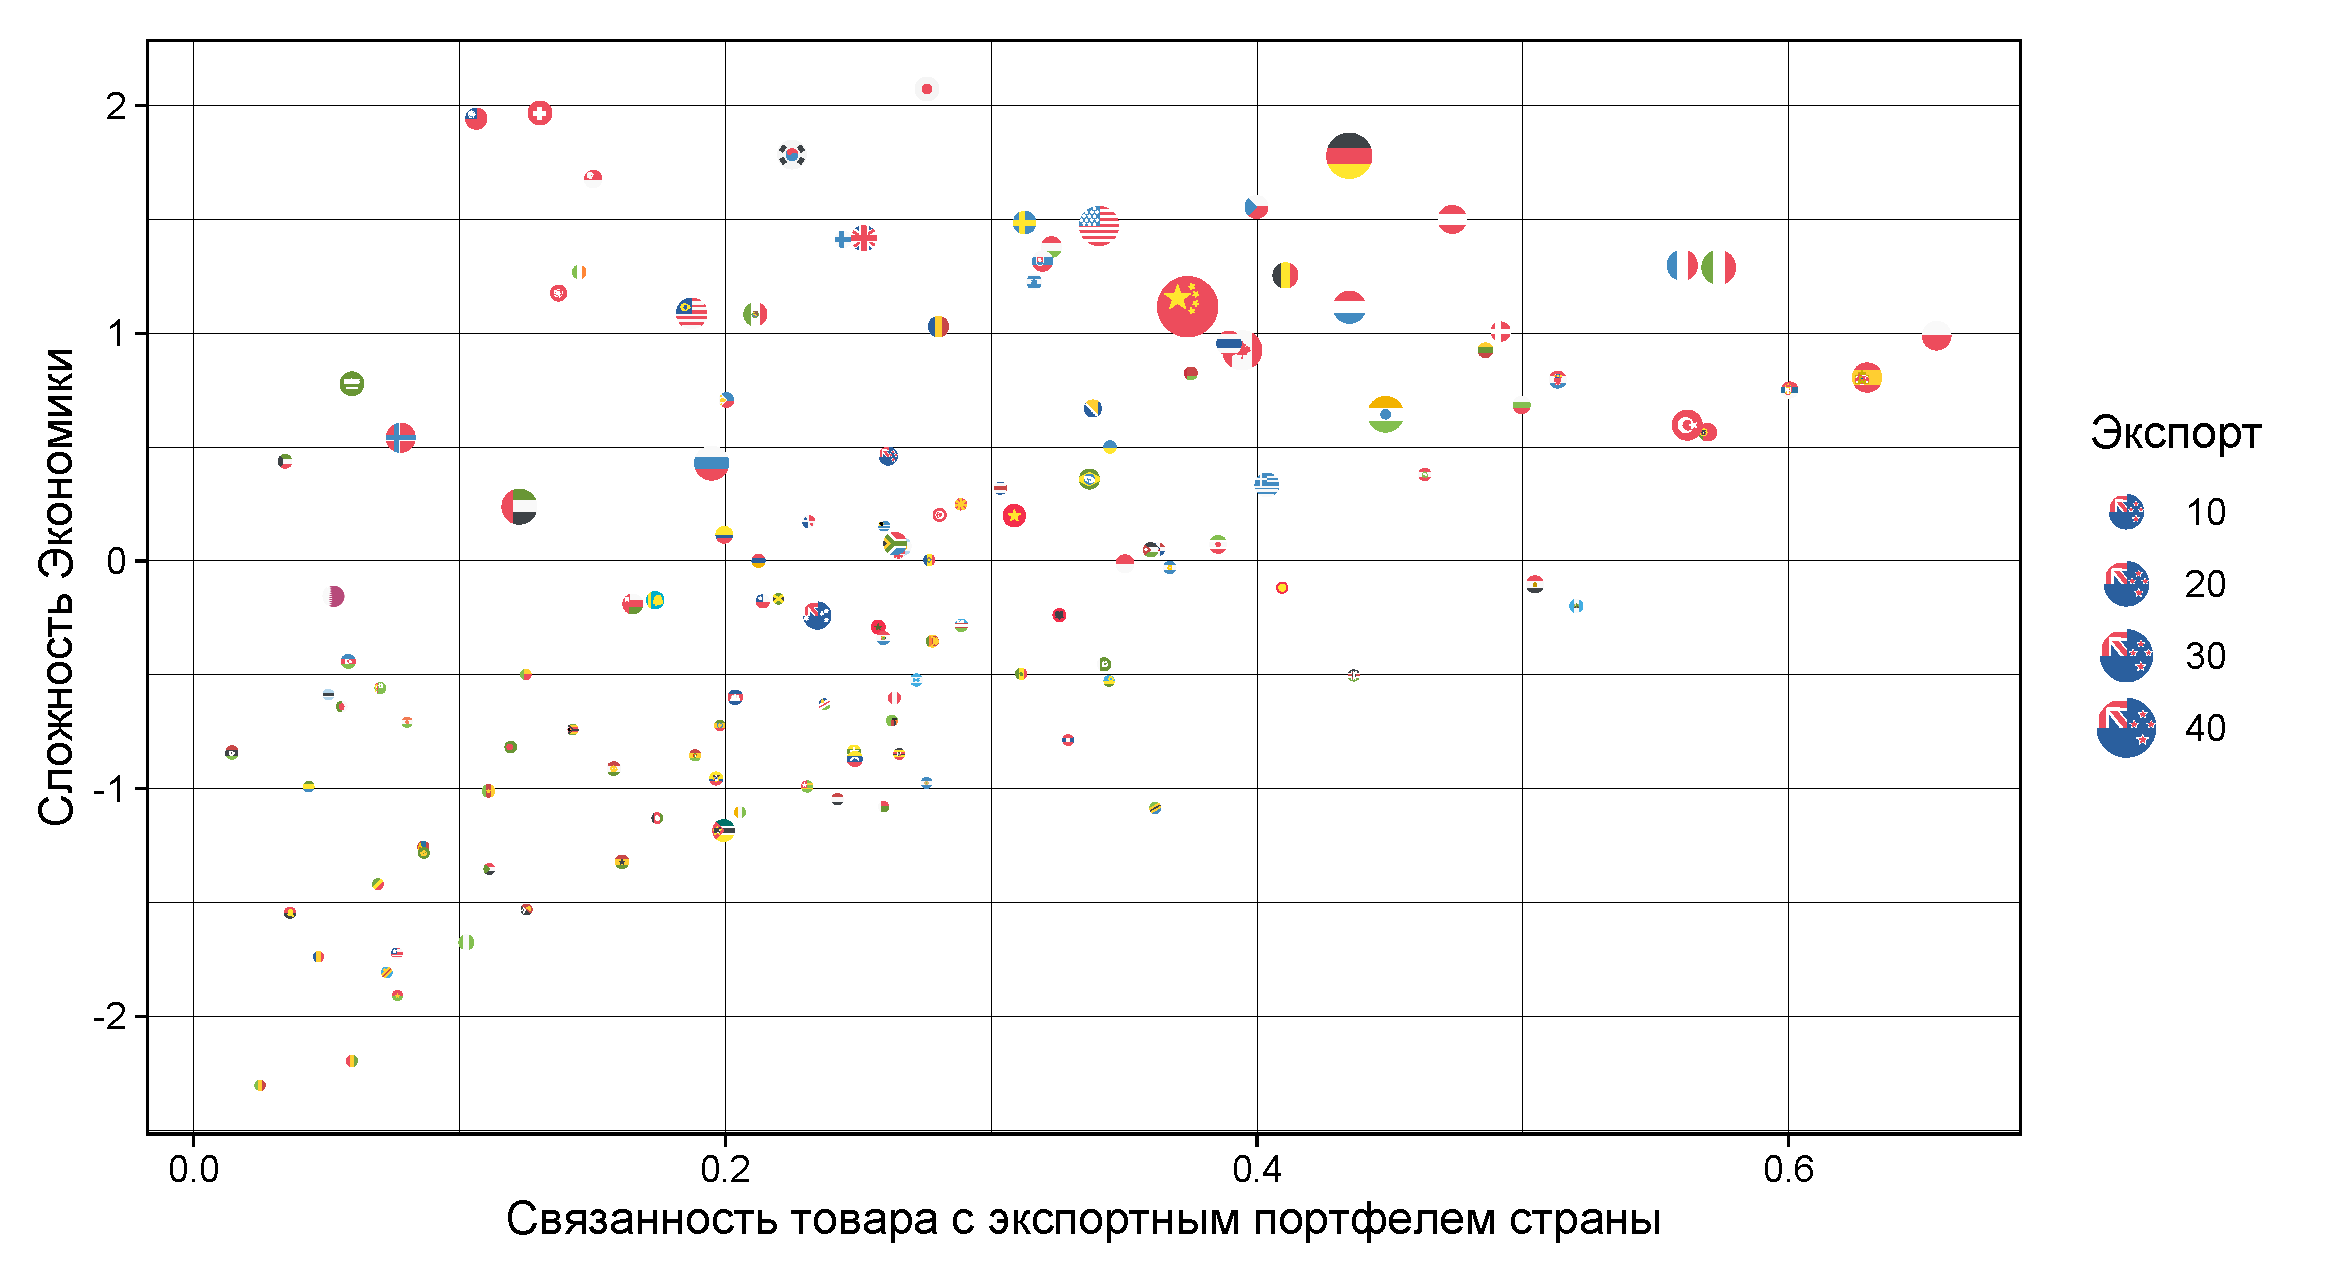
\includegraphics[width=\textwidth, height=0.8\textheight]{Plots/Recommendation/oec-plot-2.eps}
    \end{center}
\end{frame}

\begin{frame}
    \frametitle{Рекомендации\footnote{OEC}}
    \begin{center}
        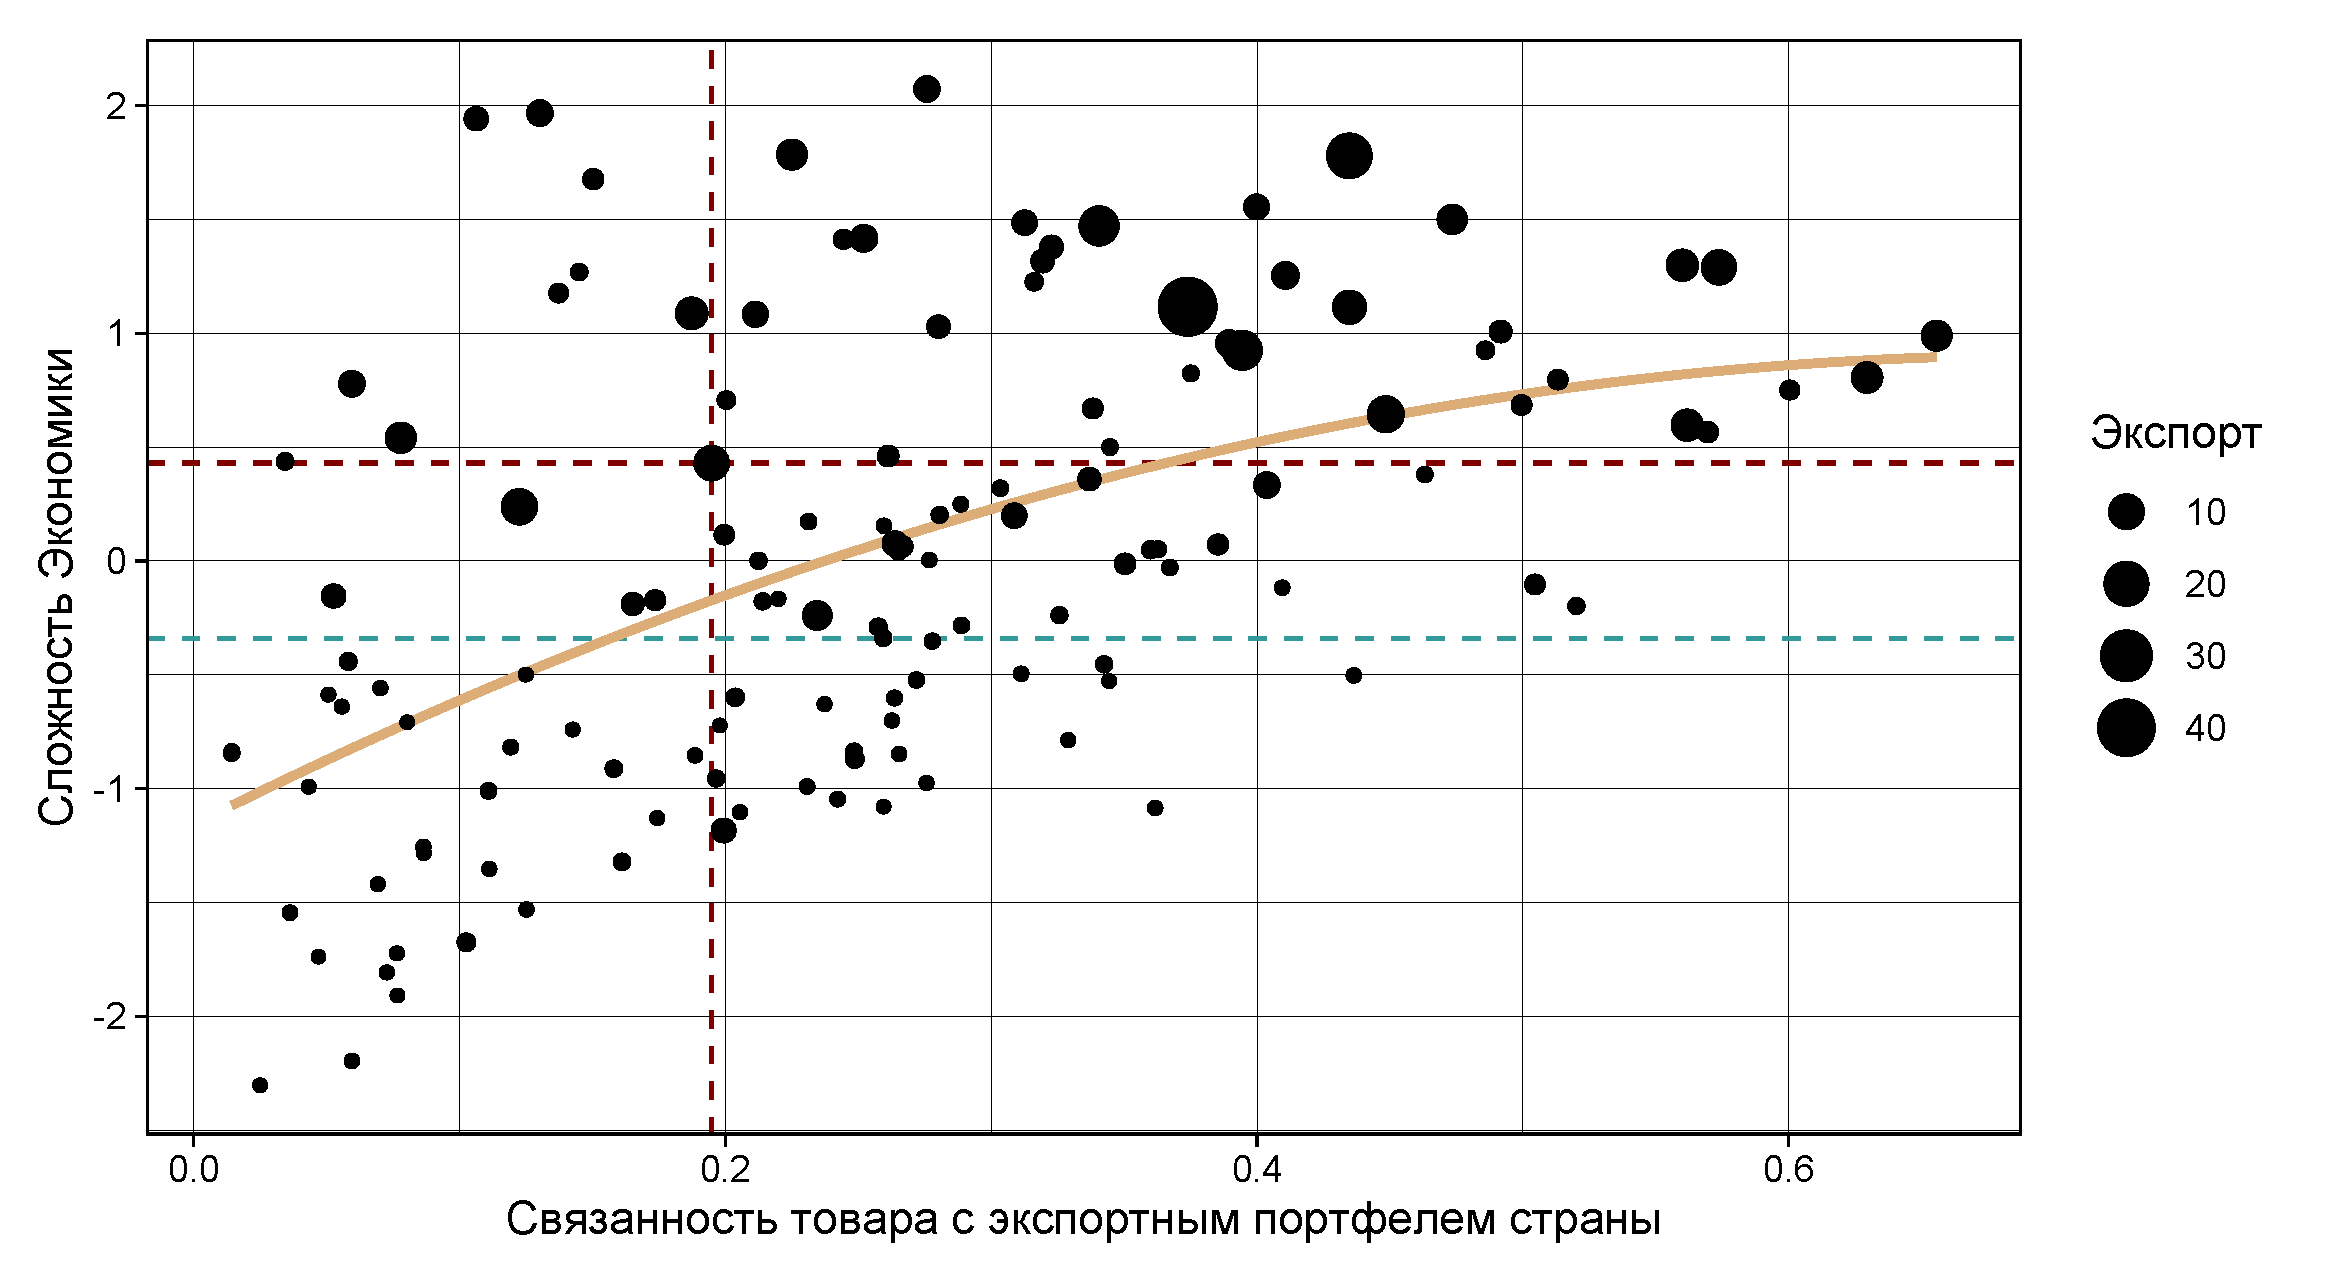
\includegraphics[width=\textwidth, height=0.8\textheight]{Plots/Recommendation/oec-plot-1.eps}
    \end{center}
\end{frame} % Рекомендации

% Заключение
\section*{Заключение}

\begin{frame}
    \frametitle{Заключение}
\end{frame} % Заключение

% Конец документа
\end{document}